\chapter{Performance}

\section{Google Lighthouse}

Google Lighthouse is an open-source, automated tool developed by Google to improve the quality of web pages. It provides audits for performance, accessibility, best practices, SEO, and progressive web apps. By running Lighthouse, developers receive detailed reports with actionable recommendations to optimize their websites. The main benefits include faster page load times, improved user experience, better accessibility compliance, enhanced search engine visibility, and adherence to modern web standards. Lighthouse can be run in Chrome DevTools, from the command line, or integrated into continuous integration pipelines to ensure consistent web performance improvements.

\section{Mobile}

\textbf{Metrics:}
\begin{itemize}
    \item First Contentful Paint - 1.7s
    \item Total Blocking Time - 20ms
    \item Speed Index - 1.7s
    \item Largest Contentful Paint - 4.4s
    \item Cumulative Layout Shift - 0.111
\end{itemize}

\begin{figure}[H] % Forces figure here
    \centering
    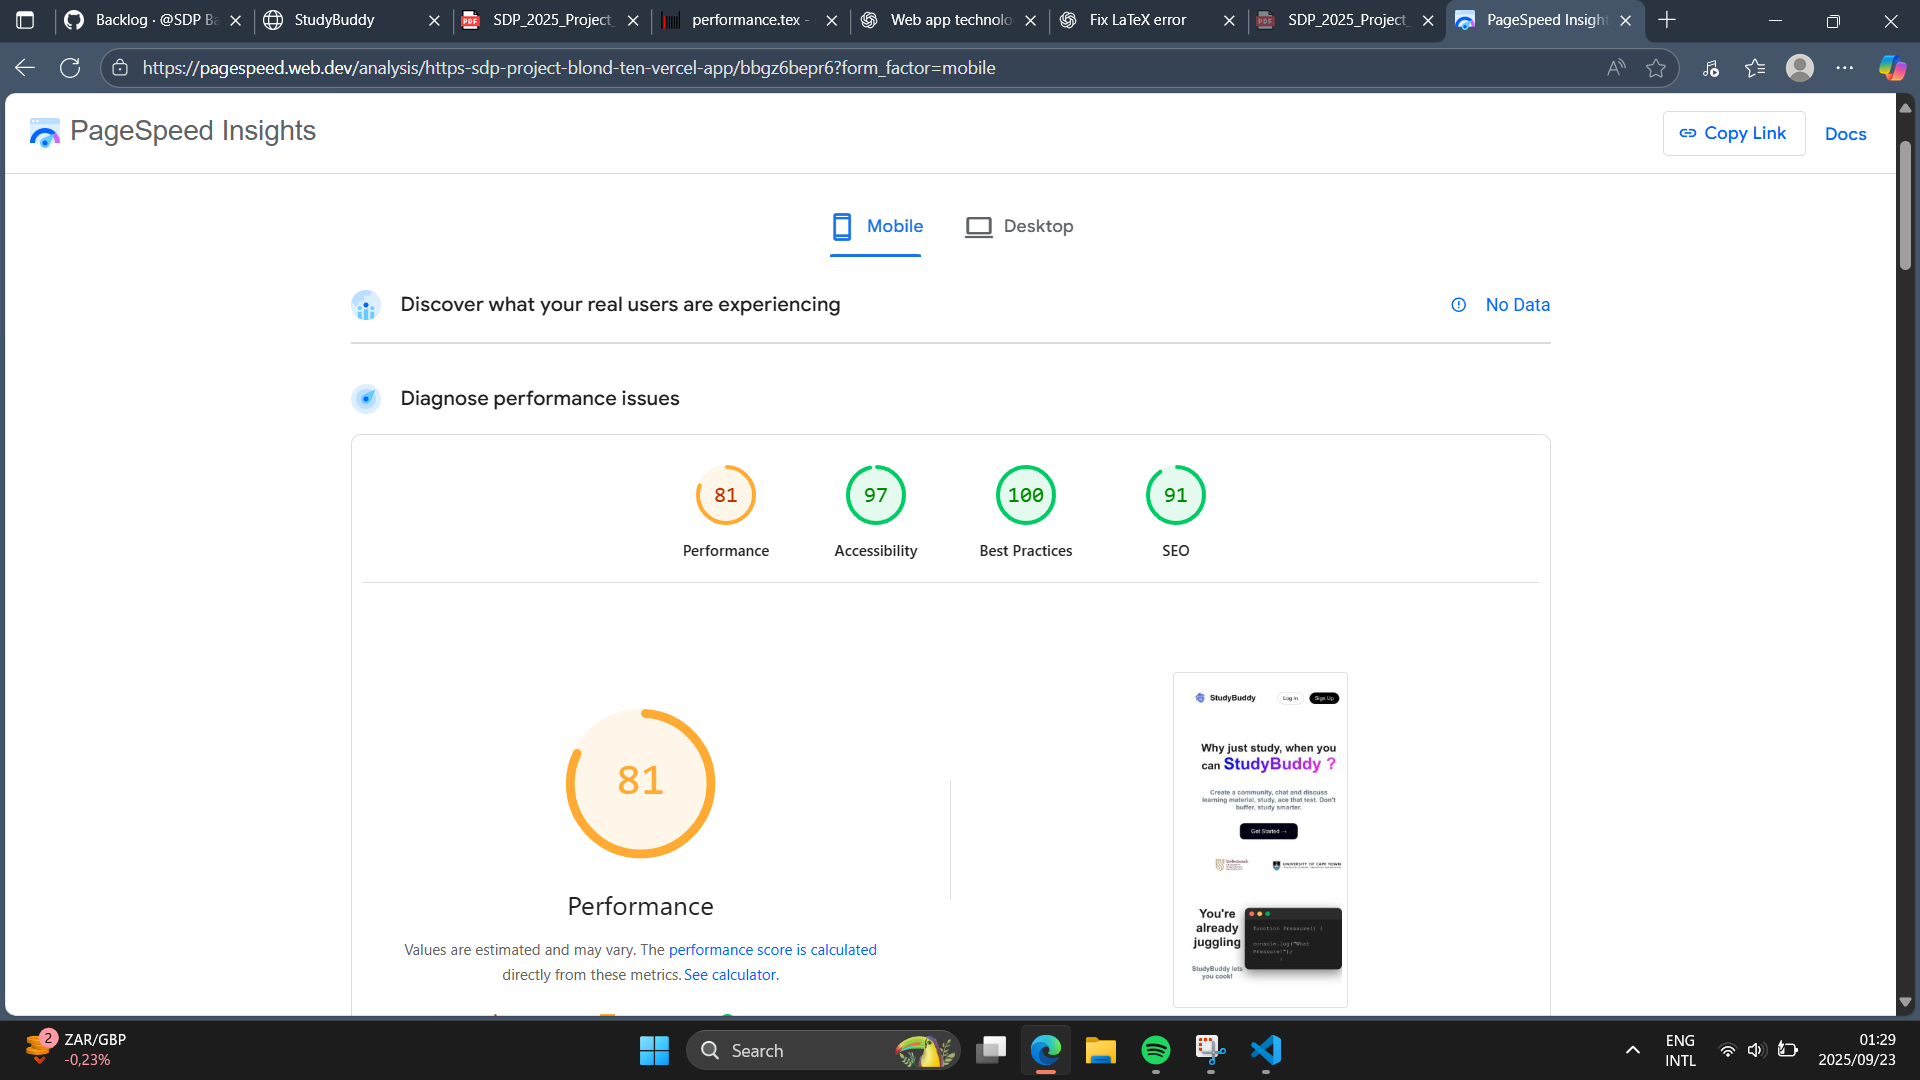
\includegraphics[width=0.8\textwidth]{mobile.png}
    \caption{How Study Buddy performs on mobile devices}
    \label{fig:mobile_performance}
\end{figure}

\section{Desktop}

\textbf{Metrics:}
\begin{itemize}
    \item First Contentful Paint - 0.4s
    \item Total Blocking Time - 0ms
    \item Speed Index - 0.4s
    \item Largest Contentful Paint - 0.8s
    \item Cumulative Layout Shift - 0.118
\end{itemize}

\begin{figure}[H]
    \centering
    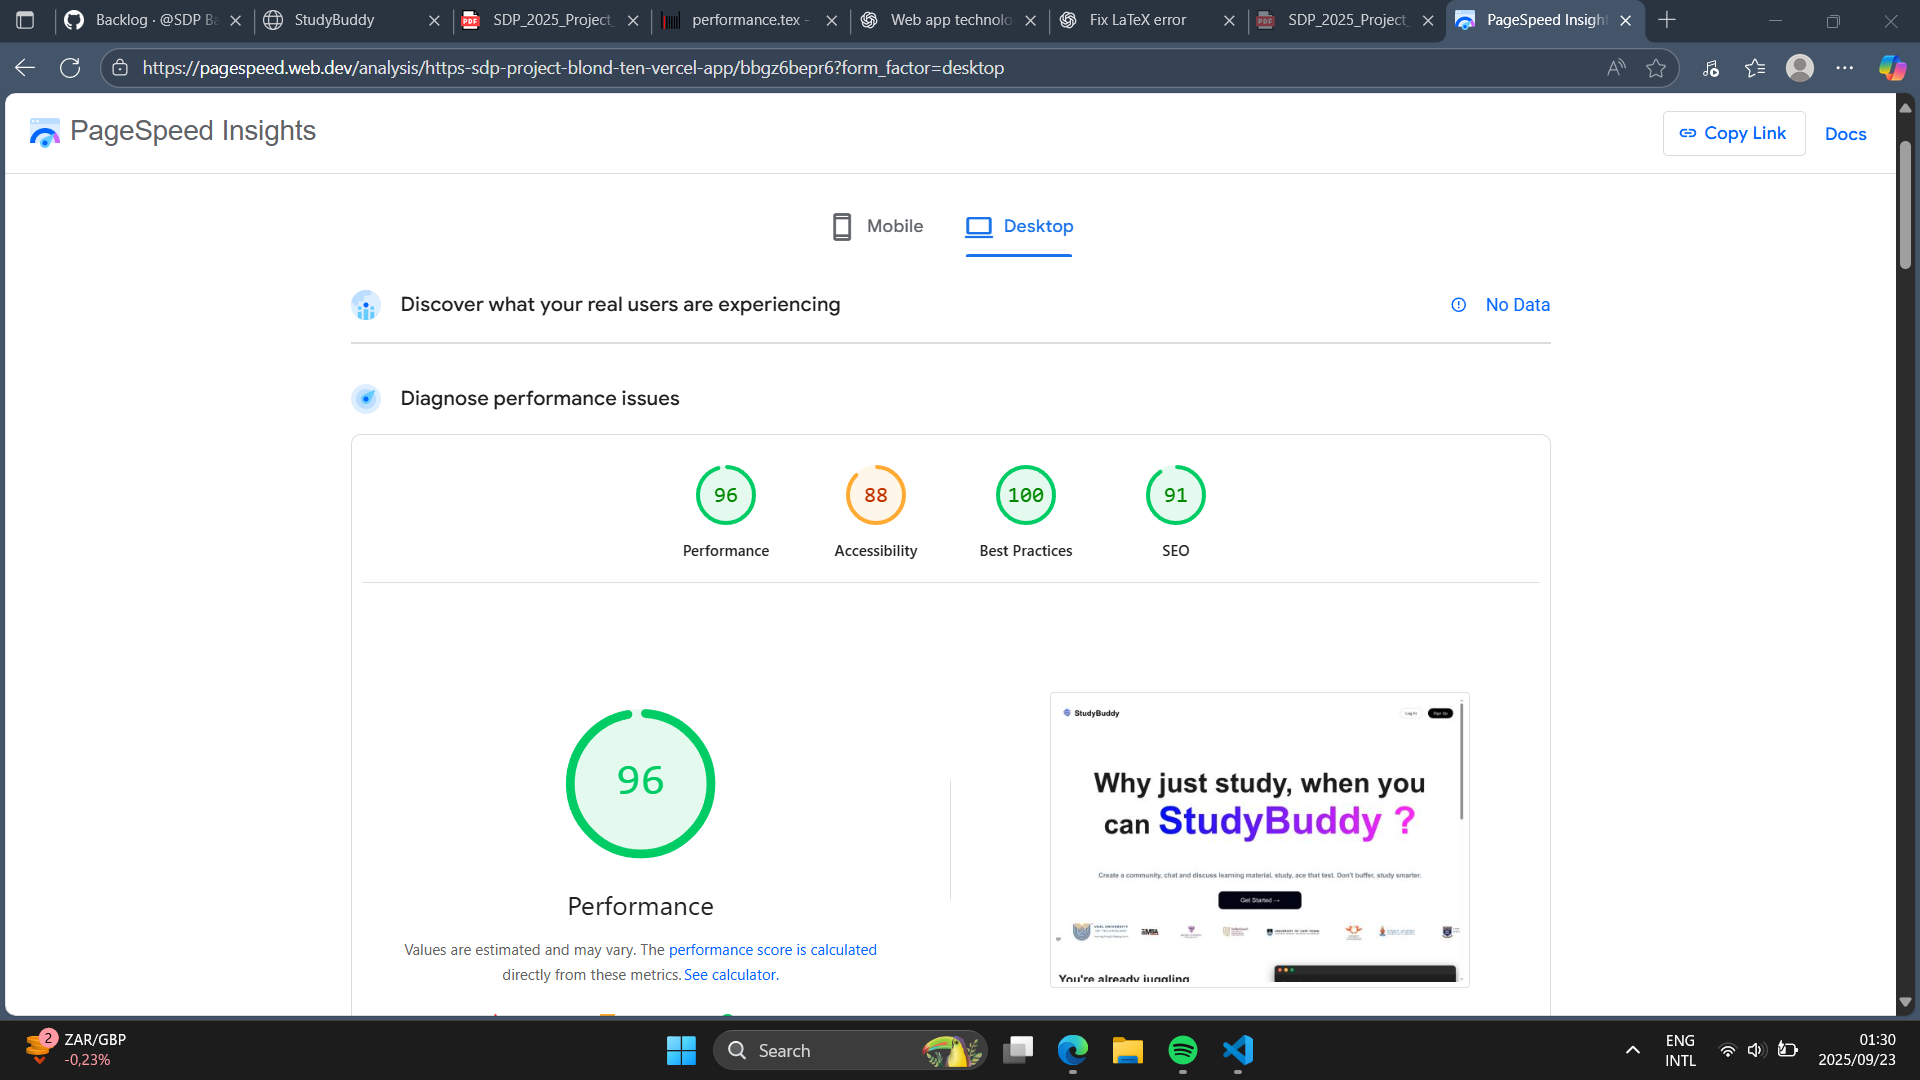
\includegraphics[width=0.8\textwidth]{desk.png}
    \caption{How Study Buddy performs on desktops}
    \label{fig:desktop_performance}
\end{figure}
